\documentclass{article}
\usepackage[letterpaper, margin=0.95in]{geometry}
\usepackage[T1]{fontenc}
\usepackage{titleps}
\usepackage{parskip}
\usepackage{booktabs}
\usepackage{graphicx}
\usepackage{xcolor}
\usepackage{microtype}
\usepackage[hidelinks]{hyperref}

\newpagestyle{ruled}
{\sethead{CMU 16-831}{Intro to Robot Learning}{Fall 2026}\headrule
  \setfoot{}{}{}}
\pagestyle{ruled}
\renewcommand\makeheadrule{\color{black}\rule[-.75\baselineskip]{\linewidth}{0.4pt}}

\begin{document}

\begin{center}
    {\Large Assignment 1: Imitation Learning} \\
    \vspace{.25cm}
    \textbf{Andrew ID:} \texttt{vawale} \\
    \textbf{Collaborators:} Claude (Anthropic), a generative AI tool, mostly used for help with
    code and drafting this report.
\end{center}

\section{Behavioral Cloning (10 pt)}

\subsection{Part 2 (1.5 pt)}

Each environment comes with two expert trajectories of 1000 steps. Table~\ref{tab:p2}
gives the mean and standard deviation of their returns.

\begin{table}[!h]
  \centering
  \caption{Mean and standard deviation of expert return over two trajectories, for each environment.}
  \begin{tabular}{cccccc}
    \toprule
    Metric/Env & Ant-v2 & Humanoid-v2 & Walker2d-v2 & Hopper-v2 & HalfCheetah-v2 \\
    \midrule
    Mean  & 4713.65 & 10344.52 & 5566.85 & 3772.67 & 4205.78 \\
    Std.  & 12.20 & 20.98 & 9.24 & 1.95 & 83.04 \\
    \bottomrule
  \end{tabular}
  \label{tab:p2}
\end{table}

\subsection{Part 3 (5 pt)}

\begin{table}[!h]
  \centering
  \caption{BC vs.\ expert return on Ant-v2 (BC works) and Hopper-v2 (BC fails). Both BC
  agents use the same settings: 5 hidden layers of width 64, learning rate
  $4\times10^{-3}$, 10000 gradient steps with minibatches of 100, trained on the 2 provided
  expert trajectories (2000 transitions), and evaluated with \texttt{eval\_batch\_size} 5000
  and \texttt{ep\_len} 1000, seed 1.}
  \begin{tabular}{ccccc}
    \toprule
    Env   & \multicolumn{2}{c}{Ant-v2} & \multicolumn{2}{c}{Hopper-v2} \\
    \midrule
    Metric & Mean  & Std.  & Mean  & Std. \\
    Expert & 4713.65 & 12.20 & 3772.67 & 1.95 \\
    BC    & 4570.02 & 61.38 & 918.30 & 257.32 \\
    \bottomrule
  \end{tabular}
  \label{tab:p3}
\end{table}

\textbf{Setup.} The two agents are identical: same network, data, training steps and
evaluation. Only the environment changes. Each mean and standard deviation covers several
rollouts, 5 for Ant and about 17 for Hopper, whose episodes end early.

\textbf{Result.} BC reaches 97.0\% of the expert on Ant, well above the 30\% target, but
only 24.3\% on Hopper.

\textbf{Why Hopper fails.} The training loss is small on both tasks ($5.5\times10^{-4}$ on
Ant, $1.7\times10^{-3}$ on Hopper), so both policies copy the expert well on the states the
expert visited. The trouble starts when the policy runs on its own. A one-legged hopper has
to balance all the time, so a small error tips it into a state the expert never visited.
The policy has no data there, the next action is worse, and the errors build up until it
falls: Hopper episodes last 297 steps on average instead of 1000. The four-legged ant is
stable, so the same small errors only slow it down, and every Ant episode ran the full 1000
steps. This compounding error is what DAgger fixes in Question~2.

\subsection{Part 4 (3 pt)}

\textbf{Question.} How does BC degrade as the amount of expert data is reduced?

\textbf{Hypothesis.} BC only knows what to do in states that appear in the demonstrations.
Less data covers fewer states, so I expected the return to hold up for a while and then
drop sharply, rather than shrink evenly.

\textbf{Setup.} Ant-v2 with the settings of Table~\ref{tab:p3}. Only the number of expert
transitions changes: 2000 (all), 1000, 500, 250 and 125, set with
\texttt{max\_replay\_buffer\_size}. The buffer keeps the most recent $N$ transitions, so
each subset is the last part of the expert data, not a random sample.

\begin{figure}[!h]
  \centering
  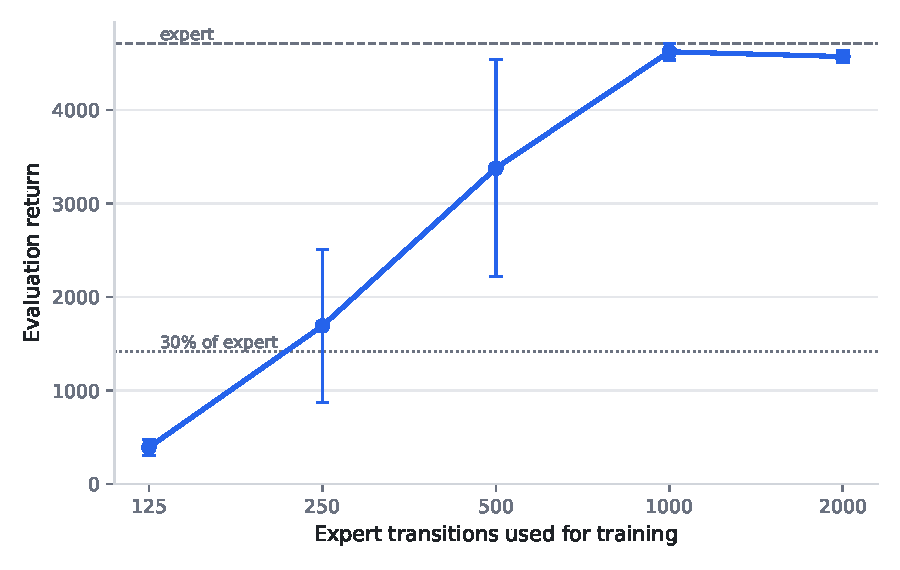
\includegraphics[width=0.6\columnwidth]{q1_part4.pdf}
  \caption{BC return vs.\ number of expert transitions on Ant-v2 (mean $\pm$ std over 5
  rollouts). Hypothesis: return drops sharply, not gradually, as expert data shrinks.
  Hyperparameter varied: amount of expert data, from 125 to 2000 transitions, with all
  other settings as in Table~\ref{tab:p3}. The result supports the hypothesis.}
  \label{fig:p4}
\end{figure}

\begin{center}
  \begin{tabular}{lccccc}
    \toprule
    Expert transitions & 125 & 250 & 500 & 1000 & 2000 \\
    \midrule
    BC return (mean) & 392.87 & 1691.08 & 3377.25 & 4620.99 & 4570.02 \\
    Std. & 87.51 & 821.39 & 1159.36 & 87.44 & 61.38 \\
    \% of expert & 8.3 & 35.9 & 71.6 & 98.0 & 97.0 \\
    \bottomrule
  \end{tabular}
\end{center}

\textbf{Result.} The hypothesis is supported. With 1000 or 2000 transitions BC stays at 97
to 98\% of the expert, and the gap between those two is within their error bars. Below 1000
it falls quickly, to 72\%, 36\% and then 8\%.

\textbf{What this shows.} The training loss moves the opposite way, from
$5.5\times10^{-4}$ with 2000 transitions down to $1.7\times10^{-4}$ with 125. The small
datasets are fitted even better, yet the agent does far worse. So the network is not
failing to learn. The data just covers too few states, and the policy is lost once it
leaves them. The large error bars at 250 and 500 agree: the ant never falls, but some
rollouts stay near familiar states and walk well while others drift off and barely move.

\subsection{Part 5 (0.5 pt)}

Zhao et~al., ``ALOHA Unleashed: A Simple Recipe for Robot Dexterity'' (CoRL 2024), use
behavior cloning to learn dexterous bimanual manipulation on the ALOHA 2 robot. The five
real-world tasks are hanging a shirt, tying shoelaces, replacing a robot finger, inserting
gears and stacking kitchen items, trained on over 26,000 demonstrations collected by human
operators teleoperating the robot through a pair of leader arms. A main risk from this
homework, covariate shift, still applies: the method is purely offline with no DAgger-style
expert correction, so the policy can fail on states the demonstrations never cover. The
paper's own failures show this, as the policy breaks down from starting configurations
absent from the data, such as a finger flipped upside down or a shirt lying face down. In
effect, the paper counters the risk with coverage rather than correction, using a very large
and diverse dataset plus 50-step action chunks, which is consistent with the Part~4 result
that BC degrades sharply as the expert data shrinks.

\section{DAgger (5 pt)}

\subsection{Part 2 (5 pt)}

\textbf{Setup.} Same two tasks and settings as Table~\ref{tab:p3}. Iteration 0 is plain BC,
so it matches Table~\ref{tab:p3} exactly. Every later iteration runs the current policy for
at least 1000 steps, has the expert label the states it visited, adds them to the dataset
and retrains. Whole rollouts are collected, so an iteration can add more than 1000 steps
when episodes end early. Over 10 iterations the dataset grows from 2000 transitions to
11000 on Ant and 12312 on Hopper.

\begin{figure}[!h]
  \centering
  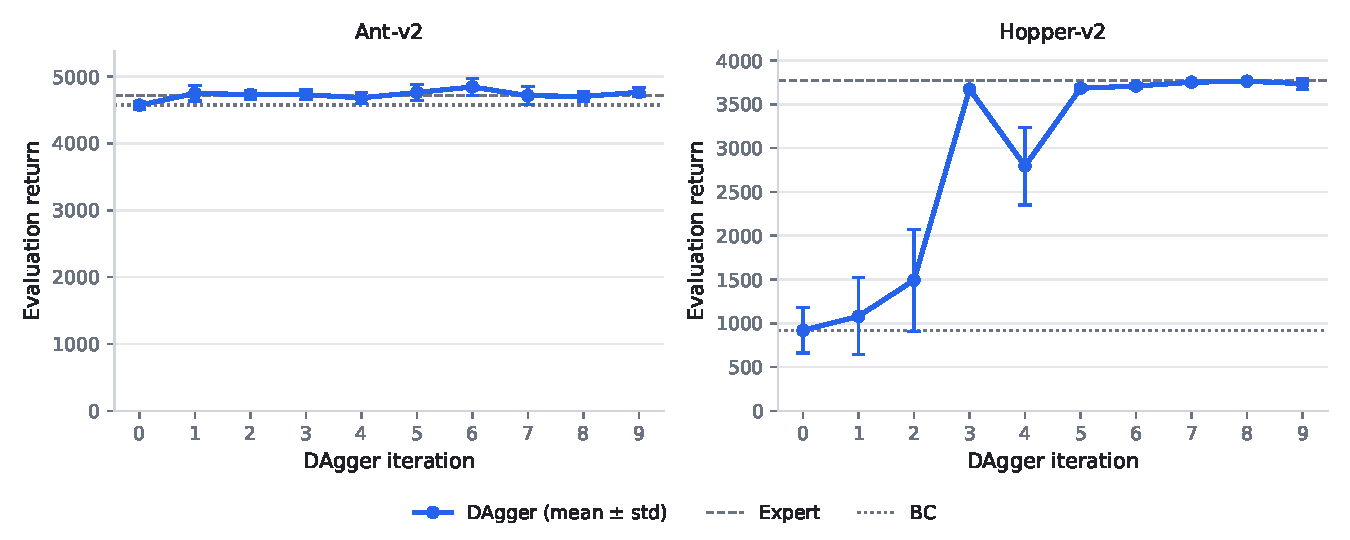
\includegraphics[width=\columnwidth]{q2_dagger.pdf}
  \caption{DAgger learning curves on Ant-v2 (left) and Hopper-v2 (right): mean evaluation
  return per iteration, with the standard deviation as error bars. The dashed line is the
  expert and the dotted line is the BC agent of Table~\ref{tab:p3}. Policy: 5 hidden layers
  of width 64, learning rate $4\times10^{-3}$, 10000 gradient steps per iteration. Data:
  2000 expert transitions at the start, plus at least 1000 new expert-labelled transitions
  per iteration for 10 iterations (whole rollouts are collected, so the count can exceed
  1000 when episodes end early). Evaluation: \texttt{eval\_batch\_size} 5000,
  \texttt{ep\_len} 1000. Both y axes start at zero.}
  \label{fig:p5}
\end{figure}

\textbf{Ant.} BC already reaches 97.0\% of the expert, so there is little left to gain.
DAgger reaches the expert level after one iteration and stays between 99\% and 103\%. The
curve is flat because it has already saturated.

\textbf{Hopper.} This is where BC failed, and DAgger fixes it. The return starts at 24.3\%
of the expert, jumps to 97.3\% at iteration 3, and saturates between 97.6\% and 99.7\% from
iteration 5 on. The average episode length goes from 297 steps to the full 1000, so the
robot stops falling. The error bars shrink from $\pm582$ at iteration 2 to about $\pm10$ at
iteration 8: at first only some rollouts survive, and in the end all of them do.

\textbf{Why it works.} In Part 3 the Hopper policy failed because its own small mistakes
led to states missing from the expert data. DAgger targets exactly those states. It lets
the policy make its mistakes, asks the expert for the right action there, and trains on the
answers, so the errors stop building up. Part 4 showed that BC is limited by which states
the data covers, and DAgger adds coverage where the policy needs it.

\textbf{The dip at iteration 4.} The return drops to 74.1\% before recovering. Each
iteration retrains on a changed dataset, so one round can come out slightly worse. The next
iteration collects data on those new failures and the policy recovers.

\end{document}
